
\documentclass[11pt,a4paper]{article}
\usepackage[left=2cm,right=2cm,top=2cm,bottom=3cm]{geometry}
\usepackage{amsmath,amsfonts,amsthm,amssymb,varioref,times, commath}
\usepackage{gensymb}
\usepackage{tikz}
\usepackage{textcomp}
\usepackage{hyperref}
\hypersetup{
 colorlinks=true,
 linkcolor=blue,
 filecolor=magenta, 
urlcolor=cyan,
}
\usepackage{lipsum}
\usepackage{epigraph}
%to resume numbering in a list
\usepackage{enumitem}
%----- arrows 
\usepackage{extarrows}

%    differential equatiosn 
\usepackage{diffcoeff}   %\diff[2]{x}{y}


%%%%%%pour ecrire en français avec les accents
\usepackage[utf8]{inputenc}
\usepackage[T1]{fontenc}
\usepackage{lmodern} % load a font with all the characters
\usepackage{units}
%%%%%%%Image-related packages
\usepackage{wrapfig}
\usepackage{float, graphicx}
\graphicspath{ {./img/} }
\usepackage{subcaption}
\usepackage[export]{adjustbox}

%%%%%%%pour faire des cadres
\usepackage{xcolor}
\usepackage{tcolorbox}
\usepackage{framed}
\usepackage{mdframed}


%%%%%%%chemistry frmulae
\usepackage{chemfig}
\usepackage{chemformula}
\usepackage[version=4]{mhchem}

% -------------- Circuits -------------------
\usepackage[european, straightvoltages]{circuitikz}

% Title & headers
\usepackage[explicit]{titlesec}
% Raised Rule Command:
% Arg 1 (Optional) - How high to raise the rule
% Arg 2 - Thickness of the rule
\newcommand{\raisedrulefill}[2][0ex]{\leaders\hbox{\rule[#1]{1pt}{#2}}\hfill}
\titleformat{\section}{\Large\bfseries}{\thesection. }{0em}{#1\,\raisedrulefill[0.4ex]{1pt}}

% pour ecrire sur +sieurs colonnes
\usepackage{multicol}
\setlength{\columnseprule}{0pt}
\setlength{\columnsep}{60pt}
% Fusion de lignes de tableaux.
\usepackage{multirow}
% Position verticale des lettres dans la ligne de tableau.
\usepackage{array}

% physics -----------------------------------------------------------
\newcommand{\To}{\longrightarrow}
\newcommand{\gpl}{\; g\cdot L^{-1}}
\newcommand{\gpmol}{\; g\cdot mol^{-1}}
\newcommand{\mpl}{\; mol\cdot L^{-1}}
\newcommand{\mps}{\; m\cdot s^{-1}}
\newcommand{\rps}{\; rad\cdot s^{-1}}
\newcommand{\kph}{\; km\cdot h^{-1}}
\newcommand{\mpss}{\; m\cdot s^{-2}}
\newcommand{\Dt}{\Delta t}
\newcommand{\vv}{\vec{v}}
\newcommand{\va}{\vec{a}}
\newcommand{\vp}{\vec{p}}
\newcommand{\vf}{\vec{F}}
\newcommand*{\Vf}[1]{\overrightarrow{F_\ensuremath{{#1}}}}
\newcommand{\es}[1]{\cdot10^{#1}}
\newcommand{\eng}[1]{\textcolor{purple}{(= #1})}
\usepackage{harpoon}
%\newcommand*{\vect}[1]{\overrightharp{\ensuremath{#1}}}
\newcommand*{\Vect}[1]{\overrightarrow{\ensuremath{#1}}}
\newcommand{\pfd}[1]{\sum \vec{F}_{ext_{#1}} &= \od{\vp_{#1}}{t} = m\cdot\va_{#1}}
\newcommand{\C}{\degree C}
\newcommand{\Delt}{\Delta t}

% --- Circuits ------------
\newcommand{\bipole}[1]{
\begin{circuitikz} \draw
(0,0) to[ #1 ] (2,0); 
\end{circuitikz} {\hspace{5mm}}}

% Chimie ---------------------------------
\newcommand{\oxo}{\ce{H3O+}_{(aq)}}
\newcommand{\eau}{\ce{H2O}_{(\ell)}}
\newcommand{\OH}{\ce{HO-}_{(aq)}}
\newcommand{\AH}{\ce{AH}_{(aq)}}
\newcommand{\A}{\ce{A-}_{(aq)}}
\newcommand{\MnO}{\ce{MnO_4^{-}}}
\newcommand{\conc}[1]{\left[{#1}\right]}
\newcommand{\couple}[2]{\ce{#1/#2}}


% Environnements ------------------------
\newcounter{exo}
\newenvironment{exo}[1][]
{\refstepcounter{exo} \begin{shaded}\noindent $\triangleright \quad$\textbf{Exercice~\theexo. #1} } { \end{shaded}}
\newenvironment{eg}
{\begin{shaded} \textbf{Exemple:} } { \end{shaded}}

\newenvironment{defn}[1]
{\begin{leftbar}\noindent \textbf{Définition :\textit{ \quad #1}} } { \end{leftbar}}

%\newenvironment{rmrq}
%{\begin{shaded} \textbf{Remarque.\quad } \itshape } { \end{shaded}}
\newenvironment{rmrq}
{\begin{mdframed}[backgroundcolor=blue!10, linewidth=0pt] \textbf{Remarque.\quad } \itshape } { \end{mdframed}}

\newenvironment{python}
{\begin{shaded} \textbf{A faire en PYTHON}\\ \itshape } { \end{shaded}}

% Shading colour -----------------------------
\definecolor{shadecolor}{gray}{0.9}

\date{}
\author{}

\renewcommand*\contentsname{Résumé}









% Title & headers 
\usepackage{fancyhdr}
\pagestyle{fancy}
\fancyhf{}
\lhead{SciPhy : Terminale spé}
\rhead{$\Phi$ - 3 : La mécanique newtonienne}
\chead{2020-28}
\rfoot{Page \thepage}
\lfoot{\textcopyright\; S Zayyani}
\renewcommand{\footrulewidth}{0.1pt}% default is 0pt

\title{\large Physique - Chapitre 3 \\ \LARGE Applications de la mécanique newtonienne :  \\ \large Les champs uniformes \& La mécanique céleste}
\date{}
\author{}

\setlength{\parindent}{0mm}
\setlength{\parskip}{2mm}

%%%%%%%%%%% For wrapfigure 
\setlength{\intextsep}{6pt}%
\setlength{\columnsep}{3pt}%



\begin{document}
\maketitle
\vspace{-1cm}
\begin{tcolorbox}[title=Notions de la classe de première à rappeler]
calcul d'une dérivée ; principe d'inertie ; vecteurs ; trigonométrie ; décompositions des forces
%\tcblower
\end{tcolorbox}
\tableofcontents

\section{Une méthode générale de résolution de problème}

Jusqu’ici nous avons retracé, plus ou moins, les premières étapes du programme de recherche de Newton, d’il y a plus de quatre siècles. On peut maintenant s’attaquer à un des problèmes principaux qui l’avaient motivé : la description du mouvement des objets dans l’univers. 

Pour cela, il faut une approche méthodologique à la résolution des problèmes de mécaniques que l'on pourra appliquer à une grande diversité de situations, soulignant que les principes derrières BEAUCOUP de phénomènes sont les mêmes, malgré les apparence qui peuvent nous tromper. 
\newpage

\subsection{La méthode}

Nous allons découper la méthode de résolution de problèmes en plusieurs étapes, afin de montrer à quel point cette approche est systématique. Voilà donc les étapes que nous allons suivre, pour chaque problème, indépendemment de la situation étudiée : 

\begin{mdframed}[backgroundcolor=blue!5]

\begin{enumerate}
    \item \textbf{Définir le système étudié : } \\
    Ceci se fait exactement comme nous l'avons déjà fait dans le cas des problèmes de conservation de quantité de mouvement. Le but ici est de pouvoir déterminer où se situé "l'extérieur" du système. 
    \item \textbf{Choisir le référentiel :} \\
    Pour nous en terminale, ce serait toujours un référentiel galiléen, c'est à dire un référentiel qui est en mouvement rectiligne uniforme. 
    \item \textbf{Choisir le repère : }\\
    Le choix du repère est essentiel pour un calcul correct. Il s'agit de choisir un repère, par exemple, cartésien, mais aussi du choix des signes pour les axes; par exemple de définir le sens gauche à droite comme positif, ou négatif.   
    \item \textbf{Faire un diagramme de bilan des forces (BDF)\eng{Free-body diagram (FBD)} : }\\
    Trouver le bon BDF est l'élément clef de la résolution du problème. L'objectif ici n'est pas un diagramme à la bonne échelle, mais plutôt l'identification des bonnes forces (extérieures au système choisi dans la première étape), et leur orientation par rapport au système d'étude. 
    \item \textbf{Décomposer le problème selon les axes du repère : } \\
    Un des points très fort de la mécanique classique est la possibilité de décomposer tout problème multidimensionnels, un plusieurs problèmes unidimensionnel, dont la résolution est beaucoup plus facile. Par exemple un problème en deux dimensions, dans un repère cartésien, peut être traité comme deux problèmes indépendants, selon $x$ et puis selon $y$. 
    \item \textbf{Appliquer le principe fondamental de la dynamique, selon chaque chaque axes. }\\
    La deuxième loi de Newton, le PFD, est l'outil principale qui nous permet d'établir un lien entre les forces agissant sur un système, et l'accélération qui en résulte; d'où l'importance d'un bon BDF. En appliquant le PFD, nous obtenons une fonction pour l'accélération du système (qui \textit{ne dépend que des forces} agissant sur le système). 
    \item \textbf{Intégrer l'accélération afin d'obtenir la fonction de la vitesse}\\
    La vitesse est la dérivée première de l'accélération (c.f. ch. 1 = cinématique du point). Une fois la fonction accélération obtenue, il suffit de trouver sa primitive qui sera la fonction vitesse. Ce processus s'appelle l'intégration. Afin de trouver une solution unique pour la fonction vitesse, par intégration, il nous faut les conditions initiales du système, notamment la vitesse initiale. 
    \item \textbf{Intégrer la fonction vitesse afin de d'obtenir la fonction position.}\\
    Comme l'étape précédente, la fonction position est la primitive de la fonction vitesse. En intégrant vitesse nous obtenons alors la fonction position. En utilisant les conditions initiales (position initiale), on obtient une fonction unique pour la position. 
    \item \textbf{Obtention des équation horaires du mouvement. }\\
    En appliquant les deux étapes d'intégration, dans chaque dimension, nous obtenons une fonction position pour chaque coordonnée. L'ensemble de ces fonctions s'appellent les équations horaires du mouvement (ou les équations paramétriques, car tout est décrit en termes d'un paramètre, ici le temps). 
\end{enumerate}
\end{mdframed}

Avant donc de s'attaquer aux premiers exemples, faisons quelques rappels rapides des notions que vous devez connaître, 
\begin{itemize}
    \item La force gravitationnelle est donnée par l'expression $\Vec{F_g} = G\dfrac{m_Am_B}{r_{AB}^2}\cdot \Vect{u_{AB}}$
    \item Dans le cas de la Terre  
    \[\Vec{F_g} = -\left(G\dfrac{m_T}{R_{T}^2}\right)m\cdot\Vect{u_{z}} \quad \Leftrightarrow \quad \Vec{F_g} = m\Vec{g} \]
    où $\Vec{g} = -G\dfrac{m_T}{R_{T}^2}\Vect{u_{z}}$ est le champs de pesanteur (un champ vectoriel), et $m_T$ et $R_T$ sont la masse et le rayon de la Terre, respectivement. 
    \item Pour être encore plus précis : $\Vec{g} = -G\dfrac{m_T}{(R_{T} + z)^2}\cdot \Vect{u_{z}}$  où $z$ est l’altitude d’un objet par rapport à la surface de la Terre. 
    \item 	Souvent, au voisinage de la surface de la Terre, on considère $\Vec{g}$  comme un champ \textit{localement uniforme} (car les variations du champ de pesanteur dues aux variations de quelques centaines de mètres d’altitude sont négligeables) ; c’est-à-dire : $\Vec{g} = -g\cdot\Vect{u_{z}}$
    \item Un objet en chute libre ne subit \textit{que} son poids. 
    \item Le repère adopté – normalement - pour l’étude des objets en mouvement dans un champ de pesanteur est cartésien.
\end{itemize}

\subsection{Un cas classique : Mouvement projectile}
Notre but dans cette partie est d'étude le mouvement d'un objet dans un champs gravitationnel uniforme (e.g. en voisinage de la surface de la Terre) en appliquant le PFD, et la méthode détaillée dans la partie précédente. 

Considérons alors le cas d’un objet de masse $m$ en chute, depuis une hauteur $h$, avec des forces résistantes négligeables. 

\begin{enumerate}
    \item \textbf{Définir le système étudié : } \\
    Le système étudié ici est simplement la masse $m$ qui est en chute libre; 
    \item \textbf{Choisir le référentiel :} \\
    Nous sommes dans le référentiel terrestre, et étant donnée la courte durée de l'événement, et la courte distance parcourue, il est supposé galiléen. 
    \item \textbf{Choisir le repère : }\\
    Le repère le plus naturel pour un mouvement pareil, est un repère cartésien. En plus, le mouvement est purement vertical, et donc, comme nous verrons, il n'y a qu'une seule dimension à considérer. 
    Nous allons donc prendre le sens vers le haut comme positif (c'est un choix arbitraire, on aurait pu choisir le sens vers le bas comme positive, et cela n'aurais rien changé au niveau du mouvement, bien sur; la différence aurait été dans l'interprétation des signes à la fin du calcul.
    \item \textbf{Faire un diagramme de bilan des forces (BDF) : }\\
    Il s'agit d'un cas très simple, car en disant que toutes forces de résistance sont négligeables, la seule force restante est le poids de la masse $\Vect{F_g}$
    \begin{figure}[H]
        \centering
        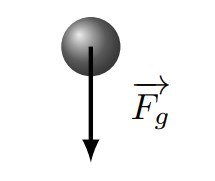
\includegraphics[width=0.1\linewidth]{imgs/p3/chutelibre.jpg}
    \end{figure}
    
    \item \textbf{Décomposer le problème selon les axes du repère : } \\
    Le mouvement dans ce cas est clairement un mouvement uni-dimensionnel, dans la direction verticale, selon $y$. Il n'y a donc que cette direction à traiter, dans l'étape suivante. 

    \item \textbf{Appliquer le principe fondamental de la dynamique, selon chaque chaque axes. }\\
    Enfin, on peut s'amuser! 
    D'après le PFD : 
    \[ \pfd{y} \]
    Ici la seule force extérieure est la force gravitationnelle, donc 
    \begin{align*}
        \Vect{F_g} &= m\va_y \\
        m\va_y &= m\Vec{g} \\
        \va_y &= \Vec{g} 
    \end{align*}
    Cela veut dire que le corps accélère, et que l’accélération est due à l’intensité de pesanteur, mais aussi que c'est dans le même sens et direction que la pesanteur. Notez bien que $\Vect{g}$ a les mêmes unités que l'accélération, c'est pour cette raison que l'on parle souvent aussi de $g$ comme l'accélération due à la pesanteur. 
    
    Comprenons aussi le sens de l'équation vectorielle $\va_y = \Vect{g} $ qui en fait est trois équations en réalité. Car si l'on décomposait cette équation selon les trois dimensions nous aurions trois équations scalaires. Il faut donc lire $\Vect{g}$ comme 
    \begin{align*}
    \Vec{g} &= \begin{pmatrix} g_x\cdot\Vec{i} \\ g_y\cdot\Vec{j} \\ g_z\cdot\Vec{k} \end{pmatrix}  = \begin{pmatrix} 0\cdot\Vec{i} \\ 0\cdot\Vec{j} \\ -g\cdot\Vec{k} \end{pmatrix}  
    \end{align*}
    et  nous avons donc, d'après le PFD :  $\begin{pmatrix} a_x\\ a_y\\ a_z\end{pmatrix} = \begin{pmatrix} 0\\ 0\\ -g\end{pmatrix} $
    
    Nous avons alors trois équations pour l'accélération dans les trois dimensions. 
    \item \textbf{Intégrer l'accélération afin d'obtenir la fonction de la vitesse}\\
    Nous avons maintenant à déterminer la vitesse en intégrant la fonction de l'accélération que l'on vient d'obtenir. Nous avons donc l’équation différentielle suivante à résoudre si l’on veut trouver les équations de mouvement : 
    \[ \od{\vv}{t} = \va   \]
    qui est en fait trois équations : 
    \[ \od{\vv_x}{t} = \va_x = \Vec{0} \quad ; \quad \od{\vv_y}{t} = \va_y = \Vec{0}\quad ; \quad \od{\vv_z}{t} = \va_z = -\Vec{g}  \]
    Si  $\od{\vv}{t} = \Vec{g}$, la détermination du vecteur-vitesse nécessite de trouver la primitive par rapport au temps de chaque coordonnée du vecteur-accélération en tenant compte des coordonnées du vecteur-vitesse initial $\vv_0 = (v_{x_0},v_{y_0},v_{z_0})$.
    
    \[\begin{Bmatrix} a_x = 0\\ a_y =0\\ a_z =-g\end{Bmatrix} \underrightarrow{\quad \text{Par Intégration}\quad }  \begin{Bmatrix} v_x(t) = v_{x_0}\\ v_y(t)=v_{y_0}\\ v_z(t)=-gt + v_{z_0} \end{Bmatrix}\]
    

    \item \textbf{Intégrer la fonction vitesse afin de d'obtenir la fonction position.}\\
    Par un raisonnement analogue à l'étape suivante (la fonction position est la primitive de la fonction vitesse que l'on vient de déterminer), par intégration on peut obtenir les équations de la position. Comme avant, afin d'obtenir une solution unique il nous faut les conditions initiales, c'est à dire la position initiale $s(0) = (x_0, y_0, z_0)$
    
        \[\begin{Bmatrix} v_x(t) = v_{x_0}\\ v_y(t)=v_{y_0}\\ v_z(t)=-gt + v_{z_0} \end{Bmatrix} \underrightarrow{\quad \text{Par Intégration}\quad }  \begin{Bmatrix} x(t) = v_{x_0}t+x_0\\ y(t)=v_{y_0}t+y_0\\ z(t)=-\dfrac{1}{2}gt^2 + v_{z_0}t + z_0 \end{Bmatrix}\]
        
    \item \textbf{Obtention des équation horaires du mouvement. }\\
    Cette série d’équations que l'on vient d'obtenir s’appelle les \textbf{équations horaires du mouvement} \eng{parametric equations}(\textit{l'équation horaire du mouvement, correspond à l’équation paramétrique d'une courbe ; le paramètre ici étant le temps}) . 
    
    Elles donnent une description générale du mouvement d’un corps en chute libre. En choisissant des conditions initiales différentes (i.e. vitesse et position initiales différentes), nous pouvons déterminer les positions différentes aux instants différents. 
\end{enumerate}

\subsection{La trajectoire}

Les équations horaires donnent l'ensemble des points occupés par le corps étudié au cours du temps, \textit{en fonction du temps}. Cet ensemble de positions dépend de la dynamique du mouvement (i.e. les forces, la loi de gravitation, etc) ET des conditions initiales : deux balles ayant exactement la même tout, dans un même champ gravitationnel, ne vont pas avoir la même trajectoire, si la position de départ n'est pas pareille; et de même si leur vitesses initiales sont différentes. 

Dans un sens donc, tout objet en chute libre dans champs uniforme (comme la pesanteur terrestre) sont absolument identiques dans leurs mouvements, aux conditions initiales près. 

Nous pouvons montrer ces différents ensembles de position différemment, grâce à l'équation de la trajectoire; la différence avec les équations horaires étant que l'équation de la trajectoire n'est pas paramétrisée par le temps. Il s'agit d'une relation de la variation d'une des coordonnées en fonction des autres : c'est une représentation de la courbe statique de la trajectoire, et non la variation de chaque coordonnée dans le temps. 

Considérons les deux conditions initiales suivantes alors : 
\begin{itemize}
    \item $v_0 = (0,0,0) $ correspondant à un corps immobile à l'instant $t=0$ ; 
    \item $v_0 = (3,0,0) $ correspondant à un corps une vitesse constante dans la direction $x$ (mouvement horizontal uniforme). 
\end{itemize}

Dans le premier cas où le corps n’a aucun mouvement initial, la trajectoire de son mouvement de chute libre sera, clairement, une ligne droite verticale, tandis que dans le deuxième cas, l'accélération due à la gravitation est vers le bas, mais le mouvement initial est horizontal, et donc la trajectoire doit être une combinaison de ces deux mouvements. Voyons alors les équations des trajectoires reflètent ce fait. 

Le mouvement ici est dans le plan vertical, généré par les vecteurs unitaires $\Vec{i}$, et $\Vec{k}$ correspondants aux coordonnées $x$, et $z$).  Il faut donc trouver l’équation $z=f(x)$, ce qui nécessite l’élimination du paramètre $t$ en combinant les équations horaires du mouvement. 

Pour cela, on se sert du paramètre $t$ présent dans les équations contenant $x(t)$ et $z(t)$, pour en faire des équivalences (simplifions le calcul ici en mettant l'origine à $s_0 = (0,0,0) $. 

C'est à dire à partir de :\begin{cases} x(t) = v_{x_0}t \quad \Leftrightarrow\quad t=\dfrac{x}{v_{x_0}}\\ z(t)=-\dfrac{1}{2}gt^2 + v_{z_0}t \end{cases}  

ce qui nous donne 
\[ z = -\dfrac{1}{2}g\left(\dfrac{x}{v_{x_0}}\right)^2 + v_{z_0}\cdot\left(\dfrac{x}{v_{x_0}}\right) \quad \Leftrightarrow\quad z = -\left(\dfrac{g}{2\cdot v^2_{x_0}}\right)x^2 + \left(\dfrac{v_{z_0}}{v_{x_0}}\right)x\]

Nous voyons clairement que l’équation $z=f(x)$ est de 2e ordre, et décrit donc une courbe parabolique. Ce qui correspond bien à la trajectoire d'un projectile dans un champs de pesanteur uniforme.

Et si nous avions d'autres conditions initiales? La méthode reste inchangée : manipuler algébriquement nos équations horaires afin d'exprimer une des coordonnées en fonctions des autres. 

\subsection{Particule dans un champ électrostatique uniforme}

Voici une autre application directe de la méthode détaillée ci-avant. La seule chose qui change est l'origine et la nature de la force agissant sur le corps. Dès l'application du PFD la force est la force exercée par le champs électrostatique, c'est à dire $F_k = q\cdot E$ où $E$ représente un champs électrostatique uniforme (comme vu en classe de première). Pour rappel, ici, $E$ est l'analogue du champs de pesanteur $g$, alors que la charge $q$ est l'analogue de la masse $m$. 

La suite est exactement pareille. 

\begin{exo}
Trouver l'expression littérale d'une charge $q$ dans un champs électrostatique uniforme $E$, située initialement à $(0,0,0)$ et immobile. 
\vspace{4.5cm}
\end{exo}

\begin{exo}
Trouver l'expression littérale d'une charge $q$ dans un champs électrostatique uniforme $E$, vertical vers le haut, et un champs de pesanteur uniforme $g$, située initialement à $(0,0,0)$ et immobile. 
\vspace{4.5cm}
\end{exo}

\section{Mécanique céleste : Lois de Kepler }

\subsection{$1ère$ loi : Loi des orbites}


\subsection{$2ème$ loi : Loi des aires}



\subsection{$3ème$ loi : Loi des périodes}

\subsection{Application : Satellites géostationnaires }

\end{document}